\chapter{Desarrollo del algoritmo}

\section{Resumen esquemático}

Para intentar resolver este problema vamos a utilizar un algoritmo que busque aproximarse al valor objetivo lo más rápido posible en su primer paso.
De esta forma, esperamos simplificar las siguientes operaciones buscando aproximaciones a un objetivo más pequeño con un menor número de valores.

\textbf{VARIABLES Y CONSTANTES:}

\begin{itemize}
	\item\textbf{Reserva:} $R=\{1,2,3,4,5,6,7,8,9,10,25,50,75,100\}$.
	\item\textbf{Candidatos:} $C=\{Seis\ valores\ elegidos\ aleatoriamente\ de\ la\ reserva\}$.
	\item\textbf{Objetivo:} $O\in\mathbb{N}:101\leq O\leq999$.
	\item\textbf{Aproximación:} Tipo de dato abstracto utilizado para buscar aproximaciones al objetivo.
\end{itemize}

\textbf{INICIO:}

\begin{itemize}
\item Cálculo de las sumas, diferencias, productos y cocientes de todas las combinaciones de candidatos.
\item Si no se ha llegado al objetivo:
	\begin{itemize}
	\item Ordenación de todas las aproximaciones por cercanía a la solución.
	\item\textbf{ITERATIVO:} Para cada aproximación obtenida:
		\begin{itemize}
		\item Cálculo de las sumas, diferencias y cocientes de todos los productos y candidatos restantes.
		\item Si no se ha llegado al objetivo:
			\begin{itemize}
			\item Ordenación de todas las aproximaciones por cercanía a la solución.
			\item Salto a ITERATIVO con los candidatos restantes.
			\end{itemize}
		\end{itemize}
	\item\textbf{FIN ITERATIVO}
	\end{itemize}
\item Si se ha llegado al objetivo:
	\begin{itemize}
	\item Devolver las operaciones realizadas para llegar a él.
	\end{itemize}
\item Si no se ha llegado al objetivo:
	\begin{itemize}
	\item Devolver la aproximación más cercana al objetivo y las operaciones realizadas para llegar a él.
	\end{itemize}
\end{itemize}

\textbf{FIN}

\pagebreak

\section{TDA ``Aproximación''}

El tipo de dato abstracto \code{Aprox} está compuesto por tres atributos:

\begin{itemize}
\item\code{int valor}\textbf{:} Entero cuyo valor es el de la aproximación.
\item\code{int candidatos[]}\textbf{:} Vector dinámico que almacena, de forma ordenada, los candidatos (no los valores intermedios) utilizados para el cálculo de \code{valor}.
\item\code{string operaciones}\textbf{:} Cadena de caracteres que almacena las operaciones utilizadas para llegar a \code{valor}.
\end{itemize}

Un ejemplo de un \code{Aprox} sería el siguiente:

\begin{lstlisting}[language=C++]
valor = 536;
candidatos = {0, 2, 3, 4}
operaciones = "(4 * 9) + (10 * 50)"
\end{lstlisting}

Consideramos que dos \code{Aprox} son iguales si tienen el mismo \code{valor} y \code{candidatos}.

\section{Cálculo de las sumas, diferencias, productos y cocientes de todas las combinaciones de candidatos}

Para calcular las sumas, diferencias, productos y cocientes de todas las combinaciones de números crearemos cuatro matrices cuadradas de tamaño $candidatos\ restantes$ en las que insertaremos los resultados de todas las respectivas operaciones con las diferentes combinaciones de candidatos.
Debido a las restricciones del reto y para no utilizar más memoria de la necesaria, suprimimos todos los valores de la diagonal principal y todos los que quedan a su derecha.
De esta forma, obtenemos la siguiente plantilla de matriz ($\times$ indica que la posición es válida y $\otimes$, que no lo es):


\begin{center}
$\begin{matrix}
[0] & \times  & \times  & \times  & \times  & \times  & \times \\
[1] & \otimes & \times  & \times  & \times  & \times  & \times \\
[2] & \otimes & \otimes & \times  & \times  & \times  & \times \\
[3] & \otimes & \otimes & \otimes & \times  & \times  & \times \\
[4] & \otimes & \otimes & \otimes & \otimes & \times  & \times \\
[5] & \otimes & \otimes & \otimes & \otimes & \otimes & \times \\
    &   [0]   &   [1]   &   [2]   &   [3]   &   [4]   &   [5]  \\
\end{matrix}$

Modelo de matriz con índices ordenados de menor a mayor
\end{center}

Conocida la forma de la matriz, conocemos los valores de cada uno de sus elementos (donde los números de cada elemento representan, respectivamente, el índice de filas y columnas):

\begin{center}
$\begin{matrix}
\times  & \times  & \times  & \times  & \times  & \times \\
1+0     & \times  & \times  & \times  & \times  & \times \\
2+0     & 2+1     & \times  & \times  & \times  & \times \\
3+0     & 3+1     & 3+2     & \times  & \times  & \times \\
4+0     & 4+1     & 4+2     & 4+3     & \times  & \times \\
5+0     & 5+1     & 5+2     & 5+3     & 5+4     & \times \\
\end{matrix}
\ \ \ \ \ \ \ \ \ \ \ \ \ \ \ \ \ \ \ \ \ \ \begin{matrix}
\times  & \times  & \times  & \times  & \times  & \times \\
1-0     & \times  & \times  & \times  & \times  & \times \\
2-0     & 2-1     & \times  & \times  & \times  & \times \\
3-0     & 3-1     & 3-2     & \times  & \times  & \times \\
4-0     & 4-1     & 4-2     & 4-3     & \times  & \times \\
5-0     & 5-1     & 5-2     & 5-3     & 5-4     & \times \\
\end{matrix}$

Matriz de sumas (izquierda) y de diferencias (derecha)

$\begin{matrix}
\times  & \times  & \times  & \times  & \times  & \times \\
1\cdot0 & \times  & \times  & \times  & \times  & \times \\
2\cdot0 & 2\cdot1 & \times  & \times  & \times  & \times \\
3\cdot0 & 3\cdot1 & 3\cdot2 & \times  & \times  & \times \\
4\cdot0 & 4\cdot1 & 4\cdot2 & 4\cdot3 & \times  & \times \\
5\cdot0 & 5\cdot1 & 5\cdot2 & 5\cdot3 & 5\cdot4 & \times \\
\end{matrix}
\ \ \ \ \ \ \ \ \ \ \ \ \ \ \ \ \ \ \ \ \ \ \begin{matrix}
\times      & \times      & \times      & \times      & \times      & \times \\
\frac{1}{0} & \times      & \times      & \times      & \times      & \times \\
\frac{2}{0} & \frac{2}{1} & \times      & \times      & \times      & \times \\
\frac{3}{0} & \frac{3}{1} & \frac{3}{2} & \times      & \times      & \times \\
\frac{4}{0} & \frac{4}{1} & \frac{4}{2} & \frac{4}{3} & \times      & \times \\
\frac{5}{0} & \frac{5}{1} & \frac{5}{2} & \frac{5}{3} & \frac{5}{4} & \times \\
\end{matrix}$

Matriz de productos (izquierda) y de cocientes (derecha)
\end{center}

Mediante el uso de este tipo de matrices nos aseguramos de considerar para la solución aquellas aproximaciones que, en el árbol de operaciones creado por el algoritmo, no tomen valores directamente de las hojas sino de operaciones ramificadas.

\begin{center}
\begin{tikzpicture}[grow'=up]
\Tree [.$825+10=835$ [.$75+11=825$ [.$9+2=11$ [.$\frac{8}{4}=2$ [.$4$ ] [.$8$ ] ] $11$ ] $75$ ] $10$ ]
\end{tikzpicture}
\begin{tikzpicture}[grow'=up]
\Tree [.$28\cdot13=364$ [.$20+8=28$ [.$\frac{100}{5}=20$ [.$5$ ] [.$100$ ] ] [.$4\cdot2=8$ [.$4$ ] [.$8$ ] ] ] [.$9+4=13$ [.$9$ ] [.$4$ ] ] ]
\end{tikzpicture}

Árbol de operaciones troncal (izquierda) y ramificado (derecha)
\end{center}

Este orden nos asegura que, siempre que el vector de candidatos esté ordenado de menor a mayor, no se producirán valores negativos en la matriz de diferencias ni resultados menores que $1$ en la matriz de cocientes.

Para realizar los cálculos sobre las matrices de forma consistente entre ejercicios, nos aseguraremos de que para cada índice \code{i} de \code{matriz}, \code{matriz[i] <= matriz[i+1]}.
Realizados los cálculos sobre ellas, debemos tener en cuenta que, aunque no se han obtenido valores negativos, sí se obtendrán valores no naturales en la matriz de cocientes, que habrá que descartar.

Teniendo esto en cuenta, almacenamos cada valor en un elemento de un vector dinámico de \code{Aprox}, que ordenaremos en el paso siguiente.

En general, el número de aproximaciones que obtenemos de esta forma se calcula recursivamente:

\begin{center}
\[\Bigg(\sum_{i=1}^{k}k-1\Bigg)-x\]

Donde $k$ es el número de candidatos y $x$, el número de aproximaciones no válidas.
\end{center}

Si durante el cálculo de los elementos de la matriz se llegara al objetivo, damos por finalizado el ejercicio.

\section{Ordenación de todas las aproximaciones por cercanía a la solución}

Obtenido el vector completo del paso anterior con las primeras aproximaciones, procedemos a ordenarlas por cercanía a la solución.
Para ello, definimos la diferencia de cada \code{Aprox} al objetivo como $|valor-objetivo|$ y los ordenamos de menor a mayor diferencia.

\pagebreak

Como consideramos antes de comenzar el ejercicio, si dos \code{Aprox} tuvieran la misma diferencia al objetivo, se considerará más cercano aquél cuyo vector de candidatos sea de menor tamaño.
En caso de que dos \code{Aprox} tuvieran el mismo \code{valor} y el mismo \code{candidatos} **no** se eliminan por considerarse duplicados, ya que existe la posibilidad de que se elijan varios candidatos iguales al inicio del ejercicio.

\section{Iteraciones posteriores}

Una vez ordenado el vector de \code{Aprox}, lo recorremos secuencialmente realizando las operaciones anteriores recursivamente hasta encontrar (o no) una combinación de operaciones cuyo resultado sea el valor objetivo.

Para construir las nuevas matrices tenemos en cuenta los candidatos que se han utilizado previamente.
Por ejemplo, si hubiéramos aproximado a $536$ con los candidatos de índice \code{0}, \code{2}, \code{3} y \code{4}, tendríamos las siguientes matrices:

\begin{center}
$\begin{matrix}
[1] & \times  & \times \\
[5] & \otimes & \times \\
    &   [1]   &   [5]  \\
\end{matrix}
\ \ \ \ \ \ \ \ \ \ \ \ \ \ \ \ \ \ \ \ \ \ \begin{matrix}
[1] & \times  & \otimes \\
[5] & \otimes & \times  \\
    &   [1]   &    [5]  \\
\end{matrix}$
\end{center}

En estos pasos debemos tener en cuenta que los valores obtenidos en las matrices aritméticas no son válidos hasta que no se hayan sumado o restestado a, multiplicado por o dividido entre el \code{valor} de la aproximación de la que partimos.

De forma recursiva, vamos realizando los mismo productos, sumas, diferencias y divisiones hasta obtener el valor objetivo o crear un nuevo vector de \code{Aprox}, que iremos recorriendo secuencialmente haciendo lo mismo hasta quedarnos sin aproximaciones.
